\begin{appendices}

\chapter{Summary}
All organisms have a genome made of DNA (deoxyribonucleic acid).
The genome can be found in nearly every cell and is the blueprint for the growth, development, maintenance and repair of the body.
It performs these functions by transcribing small pieces of DNA, the genes, from the genome and translating them to proteins.
These proteins are the tiny workhorses of the body that break down food, give bones their strength, make muscles move, let brains think, and so on.
There are many thousands of different genes and proteins with each their own task.

The genome is copied from cell to cell, and is inherited from generation to generation.
The copying process is incredibly precise, but always makes a few little mistakes.
These so-called mutations cause small differences between individuals, so that natural selection and thus evolution can take place.
Unfortunately, mutations can also cause detrimental effects, such as genetic disorders.
When the function of a gene is disrupted by a mutation, a specific disorder can arise.
For a lot of genes it is known which disorder they can cause, but for most genes we do not know what happens when they are disrupted.

In this thesis we research and develop various bioinformatics models, methods en systems to elucidate which genes and DNA differences can make people ill.
To support the research into genes, we develop a database in chapter \ref{chap:xgap}.
This database is useful for collecting all kinds of biological data.
Chapter \ref{chap:xqtl} presents software to analyze these data as an extension to this database.
This software can determine which region of the genome is responsible for diseases and other physical traits.

Organisms such as rat, worm or zebrafish allow us to perform research that would be impractical or unethical on humans.
These studies deliver valuable biological insights, but it is often remains unclear how those insights can help us to understand human disorders.
In Chapter \ref{chap:wormqtl} we report the development of an interactive database that connects research into worms to the genetics of human disease.
Despite the fact that worms do not look much like humans, they have thousands of genes that work exactly the same way as in humans.
By looking at disorders, physical traits and genes in both organisms we discover new ways to use worms for research into human diseases.

Next to understanding the genes lies the challenge to determine the harmfulness (pathogenicity) of new mutations.
Each individual carries many unique mutations no one else has.
This makes it challenging to find the causal mutation for a patient with a genetic disorder.
We can use our knowledge of the genome and evolution to predict how pathogenic new mutations are.
In chapter \ref{chap:caddmmr} we report a smart new method which predict which mutations are harmless and which cause hereditary colon cancer.
This works rather well and we make recommendations for the guideline that establishes diagnoses.

Encouraged by these results we expanded our scope from just a few to thousands of disease genes in chapter \ref{chap:gavin}.
For this, we use DNA from individuals that have no connection to severe disorders.
We compared that to disease causing mutations that were found in patients.
By crunching the numbers for every gene, it is determined when a mutation is probably disease causing.
The final result is a public website where the DNA of patients can be scanned quickly and accurately for probable pathogenic mutations.

Finally, chapter \ref{chap:frameworkforgenomics} describes how we developed a system for automated DNA analysis, including a protocol specific for genome diagnostics.
This protocol uses our new method but also the latest knowledge on mutations and genes.
Pathogenic mutations are not always responsible for the disease of a patient.
That is why the DNA of family members is used to determine if the genetic pieces of the patient truly fit.
The output is a new file format in which medically relevant information is formally expressed.
This file can be converted to a clear report in which the most important information is found at the top.

One of the advantages is that we can apply this analysis without manual work to the genomes of thousands of healthy people.
The results act as a control that tells us how often the software returns an accidental hit in each gene.
By stating this information in the final report, medical experts can focus their attention on genes with the fewest accidental hits.
This increases the speed and confidence at which a genetic diagnosis is established for the patient.

\chapter{Samenvatting}
Alle organismen hebben een genoom dat is opgebouwd uit DNA (desoxyribonucleïnezuur).
Het genoom zit in bijna elke cel en is de blauwdruk voor de groei, ontwikkeling, onderhoud en herstel van het lichaam.
Het vervult deze functies door kleine stukjes DNA, de genen, van het genoom af te schrijven en deze te vertalen naar eiwitten.
Deze eiwitten zijn de werkpaardjes van het lichaam die voedsel afbreken, botten hun sterkte geven, spieren laten bewegen, hersenen laten denken, enzovoort.
Er zijn vele duizenden verschillende genen en eiwitten met allemaal hun eigen taak.

Het genoom wordt gekopieerd van cel naar cel, en wordt overgeërfd van generatie op generatie.
Het kopieerproces is ongelofelijk precies, maar maakt altijd wel een paar foutjes.
Deze zogeheten mutaties zorgen voor kleine verschillen tussen individuen, waardoor natuurlijke selectie en dus evolutie kan plaatsvinden.
Helaas kunnen mutaties ook nadelige effecten veroorzaken, zoals erfelijke ziektes.
Wanneer de werking van een gen verstoord wordt door een mutatie kan een bepaalde ziekte optreden.
Van een hoop genen is bekend welke ziekte ze kunnen veroorzaken, maar van de meeste genen weten we niet wat er gebeurt wanneer ze verstoord worden.

In dit proefschrift onderzoeken en ontwikkelen we verscheidene bioinformatica modellen, methoden en systemen om op te helderen welke genen en DNA verschillen mensen ziek kunnen maken.
Om het onderzoek naar genen te ondersteunen, ontwikkelen we een database in hoofdstuk \ref{chap:xgap}.
Deze database is handig voor het verzamelen van allerlei biologische gegevens.
Als uitbreiding op deze database presenteert hoofdstuk \ref{chap:xqtl} software voor de analyse van deze gegevens.
Deze software kan bepalen welk gebied van het genoom verantwoordelijk is voor ziektes en andere uiterlijke kenmerken.

Dieren zoals rat, worm en zebravis stellen ons in staat om onderzoek te doen die onpraktisch of onethisch zou zijn op mensen.
Deze onderzoeken leveren waardevolle biologische inzichten op, maar het blijft vaak onduidelijk hoe die inzichten ons kunnen helpen om ziektes in de mens te begrijpen.
In hoofdstuk \ref{chap:wormqtl} rapporteren we de ontwikkeling van een interactieve database die het onderzoek naar wormen verbindt aan de genetica van menselijke ziektes.
Ondanks het feit dat wormen niet echt op mensen lijken, hebben zij duizenden genen die precies hetzelfde werken als bij mensen.
Door te kijken naar ziektes, uiterlijke kenmerken en genen in beide organismen ontdekken we nieuwe manieren om wormen te gebruiken voor onderzoek naar menselijke ziektes.

Naast het begrijpen van de genen ligt de uitdaging om de schadelijkheid (pathogeniciteit) van nieuwe mutaties te bepalen.
Ieder individu draagt vele unieke mutaties die niemand anders heeft.
Dit maakt het een uitdaging om de schuldige mutatie te vinden bij een patient met een genetische ziekte.
We kunnen onze kennis van het genoom en de evolutie inzetten om te voorspellen hoe pathogeen nieuwe mutaties zijn.
In hoofdstuk \ref{chap:caddmmr} rapporteren we een slimme nieuwe methode die voorspelt welke mutaties ongevaarlijk zijn en welke erfelijke darmkanker veroorzaken.
Dit blijkt vrij goed te kunnen en we doen aanbevelingen voor de richtlijn die diagnoses stelt.

Aangemoedigd door deze resultaten zijn we onze speelruimte gaan uitbreiden van slechts een paar tot wel duizenden ziektegenen in hoofdstuk \ref{chap:gavin}.
Hiervoor gebruiken we DNA van mensen die geen verband hebben met ernstige ziektes.
Dat vergelijken we met ziekteverwekkende mutaties die bij patienten gevonden zijn.
Met het nodige rekenwerk voor ieder gen wordt bepaald wanneer een mutatie waarschijnlijk ziekteverwekkend is.
Het resultaat is een openbare website waar het DNA van patienten snel en accuraat gescand kan worden op mogelijk pathogene mutaties.

Tenslotte beschrijft hoofdstuk \ref{chap:frameworkforgenomics} hoe we een systeem voor geautomatiseerde DNA analyse ontwikkeld hebben, inclusief een protocol specifiek voor genoom diagnostiek.
Dit protocol gebruikt onze nieuwe methode maar ook de laatste kennis over mutaties en genen.
Pathogene mutaties zijn niet altijd verantwoordelijk voor de ziekte van een patient.
Daarom wordt het DNA van familieleden gebruikt om te bepalen of het genetische plaatje bij de patient ook echt klopt.
De uitvoer is een nieuw bestandsformaat waarin medisch relevante informatie formeel wordt uitgedrukt.
Dit bestand kan worden omgezet naar een overzichtelijk rapport waarin de meest belangrijke informatie bovenaan staat.

Eén van de voordelen is dat we deze analyse zonder handwerk kunnen toepassen op de genomen van duizenden gezonde mensen.
De uitkomst hiervan dient als controle die ons verteld hoe vaak de software een toevalstreffer heeft in elk gen.
Door deze informatie in het uiteindelijke rapport te vermelden kunnen medisch experts hun aandacht richten op genen met de minste toevalstreffers.
Hiermee wordt de snelheid en zekerheid waarmee een genetische diagnose bij de patient wordt vastgesteld, verhoogd.

\chapter{Acknowledgements}

\newpage
~\\~\\~\\~\\~\\

\begin{alltt}
\ssmall
LOCUS       ACKNWLDGMNTS            1380 bp    DNA    linear    KJV 15-NOV-2017
DEFINITION  Dear friends: living beings are the result of a complex network of
            thousands of interacting genes. Likewise, a PhD thesis is the
            result of the support and collaboration of many interacting
            individuals - you! Truly, you may consider yourself the DNA of this
            thesis. I would like to sincerely thank each and every one of you
            for your kindness, brilliance and great times that allowed me to
            complete this book. Dank jullie wel!
ACCESSION   DNKWRD2017
VERSION     DNKWRD2017.1
KEYWORDS    Thanks; bedankt; gracias; merci; danke.
SOURCE      Homo sapiens (human)
  ORGANISM  Homo sapiens
            Eukaryota; Metazoa; Chordata; Craniata; Vertebrata; Euteleostomi;
            Mammalia; Eutheria; Euarchontoglires; Primates; Haplorrhini;
            Catarrhini; Hominidae; Homo.
REFERENCE   1  (bases 1 to 1380)
  AUTHORS   Van der Velde,K.J.
  TITLE     Acknowledgements
  JOURNAL   Translational software infrastructure for medical genetics
COMMENT     Special thanks goes out to my promotor Prof. Morris Swertz, for
            providing me with many interesting projects, fruitful
            collaborations, and opportunities to try out all kinds of ideas.
            Dear Morris, your energy, ambition and always positive "can do"
            attitude has been a real driver and great inspiration. Cheers!
            I would also like to express my gratitude to my other promotores,
            Prof. Richard Sinke and Assistant Prof. Yang Li, as well as Prof.
            Cisca Wijmenga and Prof. Ritsert Jansen. Your clever insights,
            constructive feedback and incredible commitment has taken my work
            to the next level. Furthermore, Prof. Rolf Sijmons and Prof. Lude
            Franke have been important sources of inspiration and wild ideas
            for which I owe them my thanks. I am also grateful for the help
            from our editors Kate and Jackie. You turn what looks like English,
            into English. Last but not least, I want to thank my paranymphs
            Freerk and Bart, and everyone who contributed in their own way
            including friends, past and present colleagues, students and
            family. I hope I managed to include all your names in the 'DNA
            code' below. Lieve papa, mama, Lianne en Misha, dank voor jullie
            steun en interesse in mijn werk. Lieve Annelies, dank voor je
            verhelderende blik, creativiteit en het aanhoren van oefenpraatjes.
FEATURES             Location/Qualifiers
     source          1..1380
                     /organism="Homo sapiens"
                     /mol_type="acknowledgemental DNA"
                     /db_xref="taxon:9606"
     mRNA            join(1..1380)
                     /gene="YOU"
                     /product="THESIS"
ORIGIN
        1 g\textbf{richard}at cc\textbf{mieke}tcc at\textbf{paul}atac a\textbf{herman}acg g\textbf{lionel}tat ct\textbf{ate}ccacc
       61 \textbf{rosalie}tca ggt\textbf{aarne}tt aga\textbf{japke}tc t\textbf{erwin}caac aacg\textbf{douwe}g aac\textbf{gertjan}
      121 cat\textbf{kate}tgc \textbf{john}cgacat gag\textbf{helene}a cag\textbf{gerben}t tag\textbf{jonne}gt atc\textbf{martijn}
      181 \textbf{luuk}gtcgag agttac\textbf{jan}a agct\textbf{birgit} aaa\textbf{sebo}acg ag\textbf{rene}cagt a\textbf{henriette}
      241 gtcag\textbf{juha}c tctgc\textbf{linni} \textbf{machiel}atc t\textbf{lennart}ga agcc\textbf{sander} gctg\textbf{lude}aa
      301 g\textbf{trijnie}tt ctac\textbf{ellen}t aagggt\textbf{jos}g gataa\textbf{tessa} cat\textbf{susanne} \textbf{janneke}cat
      361 c\textbf{menno}cgtg c\textbf{henk}aagac caag\textbf{connor} aacc\textbf{floris} g\textbf{annique}cc aata\textbf{salome}
      421 gac\textbf{chao}aac at\textbf{carin}atg t\textbf{edgar}aaca tatt\textbf{peer}ta g\textbf{patrick}ga ta\textbf{annelies}
      481 ta\textbf{nicolien} cctcg\textbf{cleo}a \textbf{xander}aaat aat\textbf{roan}aaa cc\textbf{mentje}gc c\textbf{opaenoma}a
      541 \textbf{jacques}cac t\textbf{jonathan}g \textbf{laurent}tca tta\textbf{harmen}t tataat\textbf{ger}c ag\textbf{robin}aaa
      601 \textbf{arjen}cagaa cg\textbf{michiel}c a\textbf{niek}aaaat t\textbf{basten}atc c\textbf{cisca}acta t\textbf{pieter}ata
      661 attc\textbf{george} a\textbf{marten}aag \textbf{klazien}acg c\textbf{ruggero}ga a\textbf{charlie}aa a\textbf{marielle}a
      721 \textbf{jingyuan}aa a\textbf{david}gaac a\textbf{robert}acg cgt\textbf{mariska} cat\textbf{sophie}a gaactt\textbf{leon}
      781 t\textbf{sipko}tggc aa\textbf{despoina} t\textbf{mario}tcgc g\textbf{tommy}tcac \textbf{marcjan}aaa taaatt\textbf{daan}
      841 \textbf{joke}ttggca actta\textbf{fleur} t\textbf{tom}gtttcc tcttc\textbf{joris} \textbf{matthieu}ga gc\textbf{eddy}agta
      901 ctc\textbf{pjotr}ga \textbf{jackie}gccc \textbf{alain}tgtct ca\textbf{andrew}ag a\textbf{peter}atgt a\textbf{sven}ataat
      961 a\textbf{miente}ccc \textbf{marieke}atc gt\textbf{sido}aggt atgg\textbf{wesley} ttaaa\textbf{yang}g \textbf{kristin}ata
     1021 gc\textbf{wim}atctc c\textbf{ingrid}aca acctca\textbf{bart} a\textbf{danny}agct \textbf{johanneke}c cttg\textbf{morris}
     1081 ccg\textbf{martin}a gagtcg\textbf{bote} \textbf{jip}ccctcct ttgtc\textbf{thom}g a\textbf{freerk}gta \textbf{marloes}att
     1141 ttcact\textbf{kim}t t\textbf{dennis}tca \textbf{mark}tatgag aact\textbf{rob}tat t\textbf{adriaan}tt ctta\textbf{edith}t
     1201 t\textbf{ritsert}ct t\textbf{alex}tactc tcac\textbf{erik}at c\textbf{rolf}ctgta gt\textbf{frank}gat tgacac\textbf{hans}
     1261 tgcaa\textbf{edwin} cagcc\textbf{misha} a\textbf{wietze}cca t\textbf{lianne}cac \textbf{rudi}tagaag \textbf{konrad}aaca
     1321 gaaca\textbf{joel}a t\textbf{martine}ta ct\textbf{jakob}taa tagaa\textbf{elisa} aaat\textbf{koen}ta \textbf{jelko}tatct
//
\end{alltt}



\chapter{About the author}

\begin{wrapfigure}{r}{0.33\textwidth}
  \begin{center}
    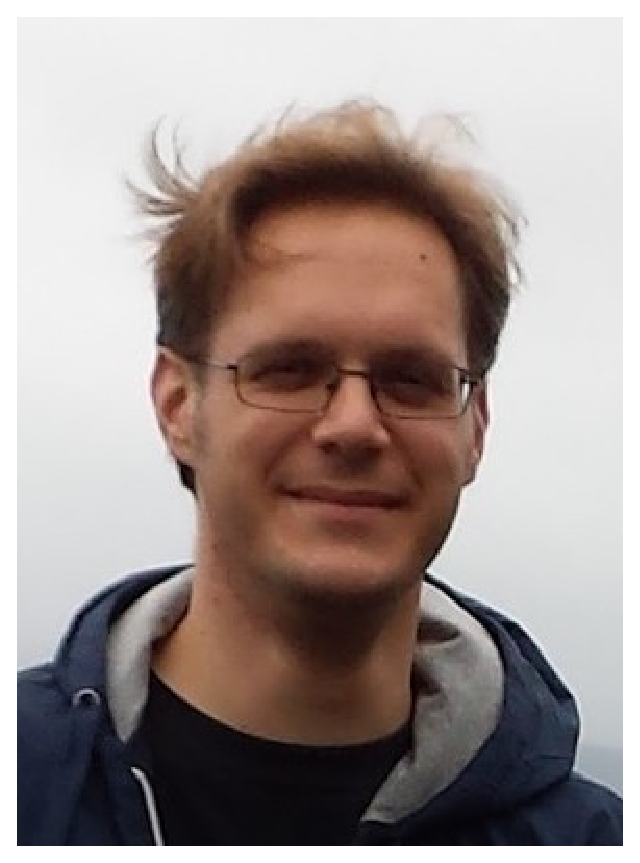
\includegraphics[width=0.33\textwidth]{img/joeri2}
  \end{center}
\end{wrapfigure}
Kasper Joeri van der Velde was born on May 24th 1986 in Drachten (municipality of Smallingerland), The Netherlands.
He completed his bachelors Bioinformatics in 2008, graduating on pathway visualizations of kinase activity at the Groningen Bioinformatics Centre in collaboration with the UMC Groningen dept. of Cell Biology.
He continued to work on MOLGENIS software infrastructure for multi-omics research in Arabidopsis, mice and C. elegans at the Groningen Bioinformatics Centre.
In 2012 he started as a PhD student at the UMC Groningen dept. of Genetics, working on new methods for downstream clinical analysis of next-generation sequencing data in the group of Morris Swertz.
Amongst a unique crowd of clinicians, software developers, geneticists, parallel computing experts, wet-lab technicians and statisticians, he aims to discover new ways to revolutionarize the speed, yield and applications of genome interpretation for medical genetics, powered by a wealth of untapped resources available in the public domain.

\chapter{List of publications}

\begin{enumerate}
\item Global genetic robustness of the alternative splicing machinery in Caenorhabditis elegans. Li Y, Breitling R, Snoek LB, \textbf{van der Velde KJ}, Swertz MA, Riksen J, Jansen RC, Kammenga JE. Genetics. 2010 Sep;186(1):405-10. doi: 10.1534/genetics.110.119677. Epub 2010 Jul 6.
\item OntoCAT – a simpler way to access ontology resources. Adamusiak T, Burdett T, \textbf{van der Velde KJ}, Abeygunawardena N, Antonakaki D, Parkinson H, and Swertz M. OntoCAT – a simpler way to access ontology resources. Nature Precedings. 2010. doi: 10.1038/npre.2010.4666.1
\item The MOLGENIS toolkit: rapid prototyping of biosoftware at the push of a button. Swertz MA, Dijkstra M, Adamusiak T, \textbf{van der Velde JK}, Kanterakis A, Roos ET, Lops J, Thorisson GA, Arends D, Byelas G, Muilu J, Brookes AJ, de Brock EO, Jansen RC, Parkinson H. BMC Bioinformatics. 2010 Dec 21;11 Suppl 12:S12. doi: 10.1186/1471-2105-11-S12-S12.
\item XGAP: a uniform and extensible data model and software platform for genotype and phenotype experiments. Swertz MA,  \textbf{Velde KJ}, Tesson BM, Scheltema RA, Arends D, Vera G, Alberts R, Dijkstra M, Schofield P, Schughart K, Hancock JM, Smedley D, Wolstencroft K, Goble C, de Brock EO, Jones AR, Parkinson HE; Coordination of Mouse Informatics Resources (CASIMIR); Genotype-To-Phenotype (GEN2PHEN) Consortiums, Jansen RC. Genome Biol. 2010;11(3):R27. doi: 10.1186/gb-2010-11-3-r27. Epub 2010 Mar 9.
\item OntoCAT--simple ontology search and integration in Java, R and REST/JavaScript. Adamusiak T, Burdett T, Kurbatova N, \textbf{Joeri van der Velde K}, Abeygunawardena N, Antonakaki D, Kapushesky M, Parkinson H, Swertz MA. BMC Bioinformatics. 2011 May 29;12:218. doi: 10.1186/1471-2105-12-218.
\item Bioinformatics tools and database resources for systems genetics analysis in mice – a short review and an evaluation of future needs. Durrant C, Swertz MA, Alberts R, Arends D, Möller S, Mott R, Prins P, \textbf{van der Velde KJ}, Jansen RC, Schughart K. Brief Bioinform. 2012 Mar;13(2):135-42. doi: 10.1093/bib/bbr026. Epub 2011 Jul 8.
\item Modifiers of mutant huntingtin aggregation - functional conservation of C. elegans-modifiers of polyglutamine aggregation. Teuling E, Bourgonje A, Veenje S, Thijssen K, de Boer J, \textbf{van der Velde J}, Swertz M, Nollen E. PLoS Curr. 2011 Aug 12;3:RRN1255. doi: 10.1371/currents.RRN1255.
\item Observ-OM and Observ-TAB: Universal Syntax Solutions for the Integration, Search and Exchange of Phenotype And Genotype Information. Adamusiak T, Parkinson H, Muilu J, Roos E, \textbf{van der Velde KJ}, Thorisson GA, Byrne M, Pang C, Gollapudi S, Ferretti V, Hillege H, Brookes AJ, Swertz MA. Hum Mutat. 2012 May;33(5):867-73. doi: 10.1002/humu.22070. Epub 2012 Apr 4.
\item xQTL workbench: a scalable web environment for multi-level QTL analysis. Arends D, \textbf{van der Velde KJ}, Prins P, Broman KW, Möller S, Jansen RC, Swertz MA. Bioinformatics. 2012 Apr 1;28(7):1042-4. doi: 10.1093/bioinformatics/bts049. Epub 2012 Feb 3.
\item WormQTL--public archive and analysis web portal for natural variation data in Caenorhabditis spp. Snoek LB, \textbf{Van der Velde KJ}, Arends D, Li Y, Beyer A, Elvin M, Fisher J, Hajnal A, Hengartner MO, Poulin GB, Rodriguez M, Schmid T, Schrimpf S, Xue F, Jansen RC, Kammenga JE, Swertz MA. Nucleic Acids Res. 2013 Jan;41(Database issue):D738-43. doi: 10.1093/nar/gks1124. Epub 2012 Nov 24.
\item An overview and online registry of microvillus inclusion disease patients and their MYO5B mutations. \textbf{van der Velde KJ}, Dhekne HS, Swertz MA, Sirigu S, Ropars V, Vinke PC, Rengaw T, van den Akker PC, Rings EH, Houdusse A, van Ijzendoorn SC. Hum Mutat. 2013 Dec;34(12):1597-605. doi: 10.1002/humu.22440. Epub 2013 Oct 16.
\item Worm variation made accessible: Take your shopping cart to store, link, and investigate! Snoek LB, \textbf{Joeri van der Velde K}, Li Y, Jansen RC, Swertz MA, Kammenga JE. Worm. 2014 Jan 1;3(1):e28357. doi: 10.4161/worm.28357. Epub 2014 Mar 6.
\item Whole-genome sequence variation, population structure and demographic history of the Dutch population. Genome of the Netherlands Consortium (Laurent C Francioli, Androniki Menelaou, Sara L Pulit, Freerk van Dijk, ..more.., \textbf{K Joeri van der Velde}, ..more.., Paul I W de Bakker, Morris A Swertz and Cisca Wijmenga). Nat Genet. 2014 Aug;46(8):818-25. doi: 10.1038/ng.3021. Epub 2014 Jun 29.
\item Genotype harmonizer: automatic strand alignment and format conversion for genotype data integration. Deelen P, Bonder MJ, \textbf{van der Velde KJ}, Westra HJ, Winder E, Hendriksen D, Franke L, Swertz MA. BMC Res Notes. 2014 Dec 11;7:901. doi: 10.1186\-/1756-0500-7-901.
\item WormQTL\textsuperscript{HD}--a web database for linking human disease to natural variation data in C. elegans. \textbf{van der Velde KJ}, de Haan M, Zych K, Arends D, Snoek LB, Kammenga JE, Jansen RC, Swertz MA, Li Y. Nucleic Acids Res. 2014 Jan;42(Database issue):D794-801. doi: 10.1093/nar/gkt1044. Epub 2013 Nov 11.
\item BiobankConnect: software to rapidly connect data elements for pooled analysis across biobanks using ontological and lexical indexing. Pang C, Hendriksen D, Dijkstra M, \textbf{van der Velde KJ}, Kuiper J, Hillege HL, Swertz MA. J Am Med Inform Assoc. 2015 Jan;22(1):65-75. doi: 10.1136/amiajnl-2013-002577. Epub 2014 Oct 31.
\item Calling genotypes from public RNA-sequencing data enables identification of genetic variants that affect gene-expression levels. Deelen P, Zhernakova DV, de Haan M, van der Sijde M, Bonder MJ, Karjalainen J, \textbf{van der Velde KJ}, Abbott KM, Fu J, Wijmenga C, Sinke RJ, Swertz MA, Franke L. Genome Med. 2015 Mar 27;7(1):30. doi: 10.1186/s13073-015-0152-4. eCollection 2015.
\item Pheno2Geno - High-throughput generation of genetic markers and maps from molecular phenotypes for crosses between inbred strains. Zych K, Li Y, \textbf{van der Velde KJ}, Joosen RV, Ligterink W, Jansen RC, Arends D. BMC Bioinformatics. 2015 Feb 19;16:51. doi: 10.1186/s12859-015-0475-6.
\item Evaluation of CADD Scores in Curated Mismatch Repair Gene Variants Yields a Model for Clinical Validation and Prioritization. \textbf{van der Velde KJ}, Kuiper J, Thompson BA, Plazzer JP, van Valkenhoef G, de Haan M, Jongbloed JD, Wijmenga C, de Koning TJ, Abbott KM, Sinke R, Spurdle AB, Macrae F, Genuardi M, Sijmons RH, Swertz MA, InSiGHT Group. Hum Mutat. 2015 Jul;36(7):712-9. doi: 10.1002/humu.22798. Epub 2015 May 20.
\item MOLGENIS/OMX for multi-omics and personalized medicine. Morris Swertz and \textbf{K. Joeri van der Velde}. Clin Bioinforma. 2015; 5(Suppl 1): S5. Published online 2015 May 22. doi: 10.1186/2043-9113-5-S1-S5
\item SORTA: a system for ontology-based re-coding and technical annotation of biomedical phenotype data. Chao Pang, Annet Sollie, Anna Sijtsma, Dennis Hendriksen, Bart Charbon, Mark de Haan, Tommy de Boer, Fleur Kelpin, Jonathan Jetten, \textbf{Joeri K. van der Velde}, Nynke Smidt, Rolf Sijmons, Hans Hillege, and Morris A. Swertz. Database (Oxford). 2015; 2015: bav089. Published online 2015 Sep 17. doi: 10.1093/database/bav089
\item MOLGENIS/connect: a system for semi-automatic integration of heterogeneous phenotype data with applications in biobanks. Pang C, van Enckevort D, de Haan M, Kelpin F, Jetten J, Hendriksen D, de Boer T, Charbon B, Winder E, \textbf{van der Velde KJ}, Doiron D, Fortier I, Hillege H, Swertz MA. Bioinformatics. 2016 Jul 15;32(14):2176-83. doi: 10.1093/bioinformatics/btw155. Epub 2016 Mar 21.
\item GAVIN - Gene-Aware Variant INterpretation for medical sequencing. \textbf{K. Joeri van der Velde}, Eddy N. de Boer, Cleo C. van Diemen, Birgit Sikkema-Raddatz, Kristin M. Abbott, Alain Knopperts, Lude Franke, Rolf H. Sijmons, Tom J. de Koning, Cisca Wijmenga, Richard J. Sinke and Morris A. Swertz. Genome Biology. 2017, 18(1). doi:10.1186/s13059-016-1141-7
\item reGenotyper: detecting mislabeled samples in genetic data. Konrad Zych, L. Basten Snoek, Mark Elvin, Miriam Rodriguez, \textbf{K. Joeri van der Velde}, Danny Arends, Harm-Jan Westra, Morris A. Swertz, Gino Poulin, Jan E. Kammenga, Rainer Breitling, Ritsert C. Jansen and Yang Li. PLOS ONE. 2017, e0171324(2) doi:10.1371/journal.pone.0171324
\item Rapid Targeted Genomics in Critically Ill Newborns. Cleo C. van Diemen, Wilhelmina S. Kerstjens-Frederikse, Klasien A. Bergman, Tom J. de Koning, Birgit Sikkema-Raddatz, \textbf{K. Joeri van der Velde}, Kristin M. Abbott, Johanna C. Herkert, Katharina Löhner, Patrick Rump, Martine T. Meems-Veldhuis, Pieter B.T. Neerincx, Jan D.H. Jongbloed, Conny M. van Ravenswaaij-Arts, Morris A. Swertz, Richard J. Sinke, Irene M. van Langen and Cisca Wijmenga. Pediatrics 2017. Published Online September 22, 2017. doi: 10.1542/peds.2016-2854
\end{enumerate}

\chapter{Other academic activities}

\begin{table}
\footnotesize
\begin{tabulary}{\linewidth}{LL}
  Date & Activity \\
  \hline
  \rule{0pt}{2.5ex}\mbox{01-09-2012} & Participated in the GSMS Project Management course \\
  \rule{0pt}{2.5ex}\mbox{06-09-2012} & Attended the 20th Annual GBB Symposium \\
  \rule{0pt}{2.5ex}\mbox{12-09-2012} & Attended the BioSHaRE Annual Meeting, Paris \\
  \rule{0pt}{2.5ex}\mbox{27-09-2012} & Gave an oral presentation at the LFN Symposium, Wageningen \\
  \rule{0pt}{2.5ex}\mbox{08-11-2012} & Participated in the PhD Introduction Event, Ezinge \\
  \rule{0pt}{2.5ex}\mbox{19-11-2012} & Attended the Connecting Biobanks Meeting, Utrecht \\
  \rule{0pt}{2.5ex}\mbox{28-11-2012} & Participated in the course 'Introduction to HL7/DCM' \\
  \rule{0pt}{2.5ex}\mbox{03-12-2012} & Participated in the Nordic BBMRI Meeting, Tartu \\
  \rule{0pt}{2.5ex}\mbox{07-01-2013} & Talked at the ENCODE Journal Club about machine learning\\
  \rule{0pt}{2.5ex}\mbox{13-03-2013} & Visited dermatology clinic at Instytut Matki i Dziecka, Warsaw \\
  \rule{0pt}{2.5ex}\mbox{19-03-2013} & Attended the CTMM TraIT Symposium, Utrecht \\
  \rule{0pt}{2.5ex}\mbox{03-04-2013} & Gave an oral presentation at the TarGet Conference \\
  \rule{0pt}{2.5ex}\mbox{16-04-2013} & Presented a poster at the NBIC Conference, Lunteren \\
  \rule{0pt}{2.5ex}\mbox{16-04-2013} & Reviewed a paper for J. of the Am. Medical Informatics Assoc.  \\
  \rule{0pt}{2.5ex}\mbox{14-05-2013} & Received the BOSC 2013 Student Travel Award \\
  \rule{0pt}{2.5ex}\mbox{17-06-2013} & Participated in the SYSGENET MC Meeting, Prague \\
  \rule{0pt}{2.5ex}\mbox{18-06-2013} & Gave an oral presentation at the BOSC Conference, Berlin \\
  \rule{0pt}{2.5ex}\mbox{25-06-2013} & Visited the dept. of Genetics at the University of Leicester \\
  \rule{0pt}{2.5ex}\mbox{01-07-2013} & Supervised internship student Mark de Haan \\
  \rule{0pt}{2.5ex}\mbox{11-07-2013} & Reviewed a paper for Journal of Web Semantics \\
  \rule{0pt}{2.5ex}\mbox{26-08-2013} & Participated in the GOPHER/RUG PhD Day \\
  \rule{0pt}{2.5ex}\mbox{11-09-2013} & Gave an oral presentation at the BMB Meeting, Dusseldorf \\
  \rule{0pt}{2.5ex}\mbox{12-09-2013} & Presented a poster at the CTMM Annual Meeting, Utrecht \\
  \rule{0pt}{2.5ex}\mbox{04-11-2013} & Gave an oral presentation at the BioShare AM, Barcelona \\
  \rule{0pt}{2.5ex}\mbox{21-11-2013} & Attended the HandsOn Biobanks Conference, The Hague\\
  \rule{0pt}{2.5ex}\mbox{12-12-2013} & Visited several research groups at the EBI, Hinxton \\
  \rule{0pt}{2.5ex}\mbox{01-01-2014} & Supervised graduation student Pieter Dopheide \\
  \rule{0pt}{2.5ex}\mbox{01-01-2014} & Supervised graduation student Mark de Haan \\
  \rule{0pt}{2.5ex}\mbox{28-01-2014} & Talked at ADCB Journal Club about Deng \textsl{et al.} (Science) \\
  \rule{0pt}{2.5ex}\mbox{23-02-2014} & Attended the Joint RD-Connect Meeting, Heidelberg \\
  \rule{0pt}{2.5ex}\mbox{20-05-2014} & Gave an oral presentation at the HVP5 Conference, Paris \\
  \rule{0pt}{2.5ex}\mbox{31-05-2014} & Presented a poster and satellite talk at ESHG Conference, Milan \\
  \rule{0pt}{2.5ex}\mbox{01-07-2014} & Supervised graduation student Tommy de Boer \\
  \rule{0pt}{2.5ex}\mbox{20-08-2014} & Taught a course segment at UMCG Biobanking Summer School \\
  \hline
\end{tabulary}
\caption[Other academic activities, pt. 1/2]{Other academic activities, pt. 1/2.}
\label{table:appendix_activities_1}
\end{table}

\begin{table}
\footnotesize
\begin{tabulary}{\linewidth}{LL}
  Date & Activity \\
  \hline
  \rule{0pt}{2.5ex}\mbox{12-09-2014} & Written a Jan Kornelis de Cock grant proposal \\
  \rule{0pt}{2.5ex}\mbox{20-09-2014} & Participated in the GOPHER/RUG PhD Day \\
  \rule{0pt}{2.5ex}\mbox{28-10-2014} & Taught course segment at VKGL/VKGN NGS diagn., Rotterdam \\
  \rule{0pt}{2.5ex}\mbox{28-11-2014} & Presented a poster at Connecting Biobanks Conference, Leiden \\
  \rule{0pt}{2.5ex}\mbox{01-01-2015} & Supervised internship student Marieke Bijlsma \\
  \rule{0pt}{2.5ex}\mbox{19-01-2015} & Talked at ADCB Journal Club about Leiserson \textsl{et al.} (Nat. Gen.) \\
  \rule{0pt}{2.5ex}\mbox{02-02-2015} & Reviewed a paper submission for ISMB/ECCB \\
  \rule{0pt}{2.5ex}\mbox{31-03-2015} & Participated in the course 'Introd. to Genetic Epidem. Research' \\
  \rule{0pt}{2.5ex}\mbox{06-06-2015} & Presented a poster at the ESHG Conference, Glasgow \\
  \rule{0pt}{2.5ex}\mbox{11-06-2015} & Attended the GSMS PhD Development Conference \\
  \rule{0pt}{2.5ex}\mbox{25-06-2015} & Talked at the Epigenome Journal Club about DIY analysis in R \\
  \rule{0pt}{2.5ex}\mbox{01-07-2015} & Supervised graduation student Marieke Bijlsma \\
  \rule{0pt}{2.5ex}\mbox{10-07-2015} & Presented a poster at the BOSC Conference, Dublin \\
  \rule{0pt}{2.5ex}\mbox{22-09-2015} & Taught course segment at VKGL/VKGN NGS diagn., Rotterdam \\
  \rule{0pt}{2.5ex}\mbox{05-11-2015} & Talked at ADCB Journal Club about Itan \textsl{et al.} (PNAS) \\
  \rule{0pt}{2.5ex}\mbox{01-01-2016} & Supervised graduation student Mariska Slofstra \\
  \rule{0pt}{2.5ex}\mbox{01-01-2016} & Supervised graduation student Thom Steenhuis \\
  \rule{0pt}{2.5ex}\mbox{18-02-2016} & Participated in the ProjectFactory course by TOC consultants \\
  \rule{0pt}{2.5ex}\mbox{04-03-2016} & Written a BBMRI voucher on variant data sharing\\
  \rule{0pt}{2.5ex}\mbox{21-03-2016} & Participated in the course 'Publishing in English gr.c' \\
  \rule{0pt}{2.5ex}\mbox{14-04-2016} & Talked at ADCB Journal Club about Zhu \textsl{et al.} (Nat. Gen.) \\
  \rule{0pt}{2.5ex}\mbox{21-05-2016} & Presented a poster and a satellite talk at ESHG, Barcelona \\
  \rule{0pt}{2.5ex}\mbox{01-06-2016} & Reviewed a paper for The American Journal of Human Genetics \\
  \rule{0pt}{2.5ex}\mbox{03-09-2016} & Gave an oral presentation at the ECCB Conference, The Hague \\
  \rule{0pt}{2.5ex}\mbox{20-09-2016} & Taught course segment at VKGL/VKGN NGS diagn., Rotterdam \\
  \rule{0pt}{2.5ex}\mbox{11-10-2016} & Taught a course segment at MPDI TopMaster course I \\
  \rule{0pt}{2.5ex}\mbox{03-11-2016} & Talked at ADCB Journal Club about Turpin \textsl{et al.} (Nat. Gen.) \\
  \rule{0pt}{2.5ex}\mbox{19-12-2016} & Reviewed a paper for Genome Biology \\
  \rule{0pt}{2.5ex}\mbox{03-07-2017} & Visited the SciLifeLab Clinical Genomics facility, Stockholm \\
  \rule{0pt}{2.5ex}\mbox{07-09-2017} & Started to supervise graduation student Sander van den Hoek\\
  \rule{0pt}{2.5ex}\mbox{11-09-2017} & Taught course segment at VKGL/VKGN NGS diagn., Rotterdam \\
  \rule{0pt}{2.5ex}\mbox{02-10-2017} & Participated in Bioschemas Adoption Meeting at EBI, Hinxton \\
  \rule{0pt}{2.5ex}\mbox{09-10-2017} & Started to supervise internship student Peer Ketelaars\\
  \rule{0pt}{2.5ex}\mbox{16-11-2017} & Gave an oral presentation at the NASPM Conference, Høvik \\
  \hline
\end{tabulary}
\caption[Other academic activities, pt. 2/2]{Other academic activities, pt. 2/2.}
\label{table:appendix_activities_2}
\end{table}

\end{appendices}

\clearpage
\pagestyle{empty}

\noindent
\textbf{Back cover image explained}\\
The back cover shows an altered version of the Arecibo message, send out on 16 November 1974 from the Arecibo Observatory in Puerto Rico. Key numbers were updated, the antenna dish graphic left out, and it was extended for medical genetics / bioinformatics. The original transmission was broadcasted with a power of 1,000 kW towards globular star cluster M13, which it will reach in roughly 25,000 years.

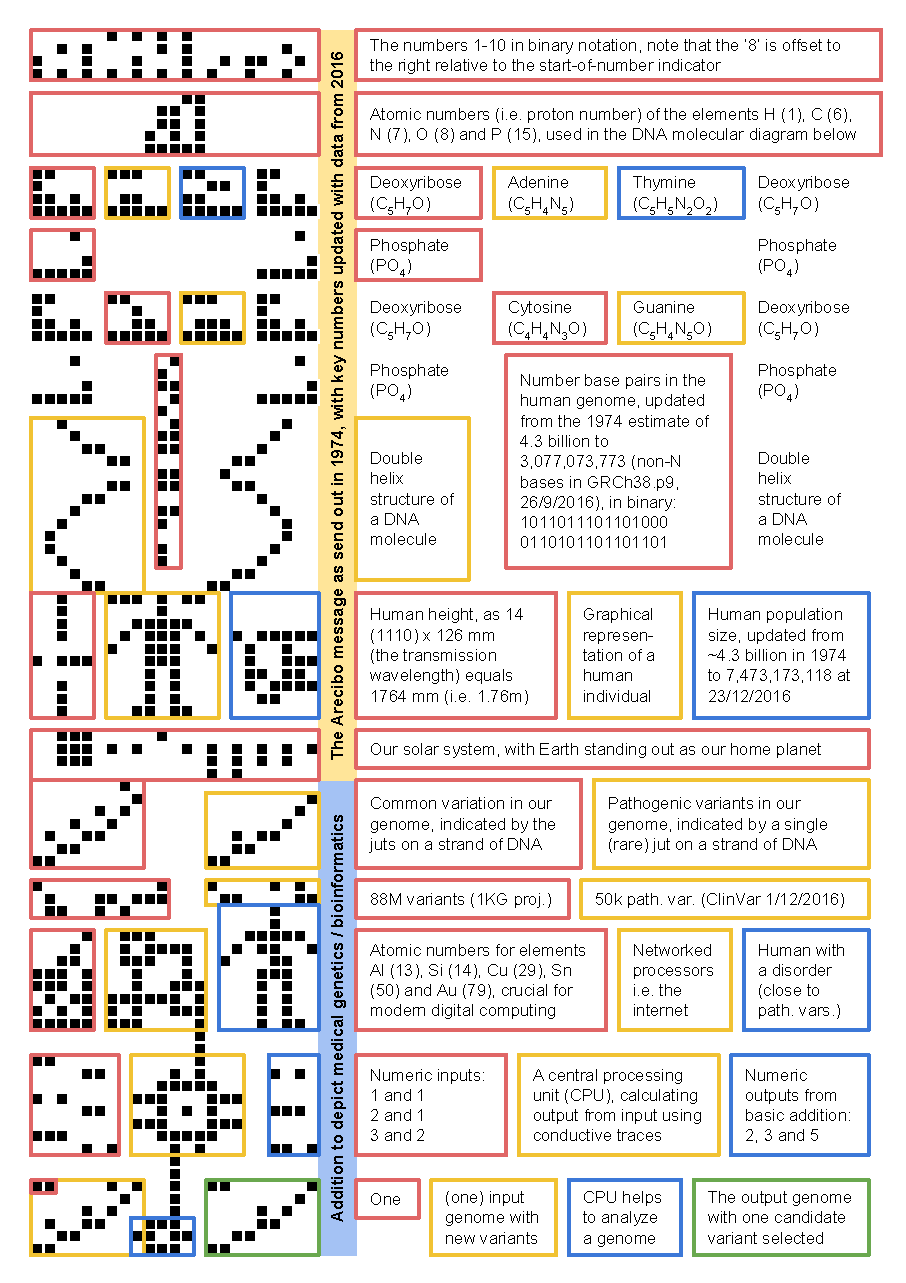
\includegraphics[scale=0.546]{img/cover_expl}
